\documentclass[twoside,12pt,titlepage,a4paper]{article}
\usepackage{url}
% kentHarvard requires natbib
\usepackage{natbib}
% add line numbers
% TODO: remove line numbers and run minted for release
\usepackage{lineno}
% \usepackage{minted}
\usepackage{etoolbox}
\makeatletter
\patchcmd{\@verbatim}
{\verbatim@font}
{\verbatim@font\scriptsize}
{}{}
\makeatother
\usepackage[final]{pdfpages}
\usepackage{xcolor}
\linenumbers
\definecolor{periwinkle}{rgb}{0.8, 0.8, 1.0}
\renewcommand{\linenumberfont}{\normalfont\bfseries\small\color{periwinkle}}
\usepackage[pass]{geometry}
\usepackage{graphicx}
\renewcommand{\baselinestretch}{1.3}
\usepackage{todonotes}
\usepackage{hyperref}
\setcitestyle{numbers}
\setcitestyle{square}

\title{Usage and structure of continuous integration as configuration?}
\author{Joseph Ling\\\vspace{10mm}
\url{jl653@kent.ac.uk} \\ \vspace{5mm}

\includegraphics[scale=0.6]{Kent_Comp_294_RGB} \\
School of Computing \\
University of Kent \\
United Kingdom \\ \vspace{10mm} \\ Word Count: around 4,400}
\begin{document}

\newgeometry{hmarginratio=1:1}    %% make layout symmetric
\maketitle
\restoregeometry              %% restore the layout

\begin{abstract}
  Continous integeration (CI) is becoming more popular as software development moves to an Agile fast paced development life cycle. Most CI is done automatically using a service which run based off configuration. Our major questions is how much is CI acutally being used? As well as how are these files being structured? We got 31,494 open source projects from Github to answer these questions. In doing so compared our results against \citet{Hilton2016} work to see if their has been a increase in usage. We found a shift in CI services being used and were able to get similar results to their study. In terms of structure we found that configuration files are written with no comments normally. We suggest at the end further research is needed to get a better understanding of this growing field.    
  \todo[]{similar is a bad word to use to describe the comparison}
\end{abstract}

\section{Introduction}
\label{Introduction}

Continous integeration (CI) is becoming more popular over the last few years. This can be seen by how major version control hosting services Github, Bitbucket and Gitlab have all started to or have been improving their CI product. In terms of research, Infrastructure as Code in \citet{Rahman2019} which does a systematic mapping of research in that area. For Continuous Integeration with \citet{Shahin2017} which does another systematic review on how it is used. These two papers demonstrate some of breadth of research that has taken place. In addition you have papers like Google's Innovation Factory: Testing, Culture, and Infrastructure \citet{Copeland2010} which demonstrate some of the depth that the papers go into.
\todo[]{google paper might not be the best one here, we want to demonstrate reading around the area here but not too include a paper which we will go into much later but is still relevant}

Continous Integeration is a process of automatically running compiling, running tests and checking that the product works. This is can be combined with Continous Delivery where the product is deployed or released after it has gone through successfully CI. 

This can get complicated quickly therefore Configuration as Code (or Infrastructure as Code) is used to configure it. The main kind of configuration format used for this is Yaml followed by Xml and Java based scripting formats.


In order to look at our first theme CI usage we looked at In Usage, Costs, and Benefits of Continuous Integration Open-Source Projects \cite{Hilton2016}. They looked closely at usage of CI as well. As we are looking at CI usage as well we are going answer the first three questions from their theme "Usage of CI". 
\begin{itemize}
  \item What percentage of open-source projects use CI?
  \item What is the breakdown of different CI services?
  \item Do certain types of projects use CI more than others?
\end{itemize}

However the two key differences is that we will be scraping a new data set for the comparison. In doing so gathering slightly more data on the repositories but not none on pull requests. As well as we didn't conduct a survey. From that additional data we are going to look more closely at the first question of What percentage of open-source projects use CI?
As we are asking the same questions, we will use their corpus to compare on what has changed over the last 4 years. 

For our second theme, structure of CI as configuration we wanted to pick structural components that would be similar between all CI files. It would have been really interesting to do a full in depth analysis of each like \citet{Gallaba2018}. However we would like to tie in how the files are structured to how they are used so won't following that style. This led to the following research questions:
\begin{itemize}
  \item What are the common errors when loading yaml configuration?
  \item How are comments used in the configuration?
  \item How are external scripts used within the configuration?
\end{itemize}

\section{Related Works}
\vspace*{-0.05in}
\subsection{Continous Integration}
\vspace*{-0.05in}

Continous Integration is frequently submitting work normally tied into a feedback loop. For example using version control daily committing changes. That then a server builds and tests the changes informing you of status of those changes. As well as providing a build for that change of the code that can be saved. In doing so it can pick up on the situation off "It works on my machine...". As the building and packaging of the code is done on a server to make sure everything integrates.

\todo[]{just because it is done on a server doesn't mean it should integerate. Althouhg it is closer to where we want to be than just talking about testing....}

An early definition of CI was written up and then updated later by Martin Fowler \cite{CI2010_MartinFowler}. A key part of the CI is that it enables makes integrate code between a team easier but it does come at a cost of...... what are you wanting to write here????



\vspace*{-0.05in}
\subsection{Usage of Continuous Integration}
\vspace*{-0.05in}

The actual usage of CI as configuration was looked at by \cite{Hilton2016}. In this they use three source of information Github repositories, Travis builds and a survey. In order to be do a more systematic study of CI usage than \cite{Vasilescu2015}. In analysing that data they found that "The trends that we discovered point to an expected growth of CI. In the future, CI will have an even greater influence than it has today." As we are looking at the same question we will use four of the research questions out of the fourteen. In order to see what difference four years has made to the growth of usage of CI.


\todo[]{rewrite this section in light of the introudction which does a better intro to this paper so we don't necessarily need to repeat ourselves here. I think we should mention it but go more in depth into some research in this area....}

\vspace*{-0.05in}
\subsection{Config as code}
\vspace*{-0.05in}

Configuration as code or Infrastructure as Code has been an increasing area of research over the last few years. There seems to be slightly more research in infrastructure as code \citet{Rahman2019}. The has been a focus on Puppet and Chef, for example in \citet{Sharma2016} looks at code quality by the measure of "code smell" of Puppet code. This tackles the problem by defining by best practices and analyzing the code against that. In the case of \citet{Cito2017} it uses the docker linter in order to be able to analyse the files. 
For the CI systems we pick we will look into the tooling around that to aid the analysis.


\section{Methodology}
\label{methodology}

% In order to get repositories with CI/CD configuration from Github we have a number of approaches. The first is too use the search for particular files but this is limited to only 1000 results. The alternative is to search for repositories and we bypass the 1000 result limit to an extent by getting results for every 'star' count (stars are used to like or upvote a repository). Although this will be giving us a lot of results it will still only be a sample of the population but will give us a wider range of results. As their is rate limiting multiple Github api keys can be used to speed up the scraping of data (Ghtorrent could also be used to speed up the process I think).

% After we have got a repository we need to get the CI/CD files from it. This is fairly easy as the CI/CD systems normally require a strict naming convention and location within the repository. However as most of them are yaml based you can have ".yml" and ".yaml" and users can use all sorts of mixtures of upper and lower case. We try to account for this but won't get every scenario. This combined with the fact that we are only looking for top configuration files based on \cite{Github2017} along with Github actions and Azure pipelines. Is why we also check repositories for their ReadMe.md file to check if it has a build tag.

% \begin{figure}[h]
%   \centering
%   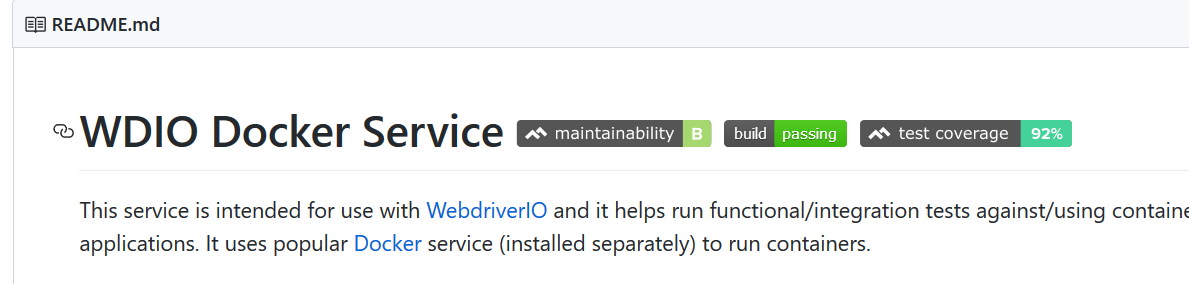
\includegraphics[scale=0.5, width=\textwidth]{2020-01-30-08-29-04.png}
  
%   \caption[alt text]{Example of CI tag for Github ReadMe}
%   \label{ExampleGithubReadme}
% \end{figure}

% \todo[size=\scriptsize]{where did this image come from?? reference it man}

% In doing so it should give a wider net when sampling and help to understand when a CI system is either not using configuration as code or using a different CI system.

% Tooling for the configuration files, we looked into Travis, Github Actions and Jenkins to work out whether or not it could aid in the research or not. As a key part of understanding the first relies on knowing whether or not it is valid. 
% In terms for Travis there is currently two parsers to validate the configuration. One which is depracted since 2017 \cite{TravisYamlParserOld2017} the other which is currently in development \cite{TravisYamlParserNew2020}. Both didn't provided the necessary results with the most recent one not being able to handle default fields.
% For Github Actions as it's still a new tooling for it hasn't been developed outside of the Github editor web page \cite{Github2019ForumPost}.
% For Jenkins which is older solution allows validation through http/ssh request to the Jenkins server (Gitlab follows this style as well) \cite{JenkkinsDocs2020} \cite{GitlabDocs2020}. This could work well although would require setting up a server for each configuration type and might not validate if varaibles from the config aren't defined on the server. As well as it would be best to be able to validate them all or none of them in terms of being able to compare results easily.





Initially the project started of as a small piece of research that would aid looking into how visualise CI systems. Therefore the initial scraping script was a quick hack to try and get some data initially. This meant that as we were not initially trying to get lots of data we did not decided to use Ghtorrent (REFERENCE). However as it quickly started to want to gather more data and look at different questions it started to form into this paper. 

\begin{figure}[!htbp]
  \centering
  \begin{minipage}{.48\textwidth}
    \centering
    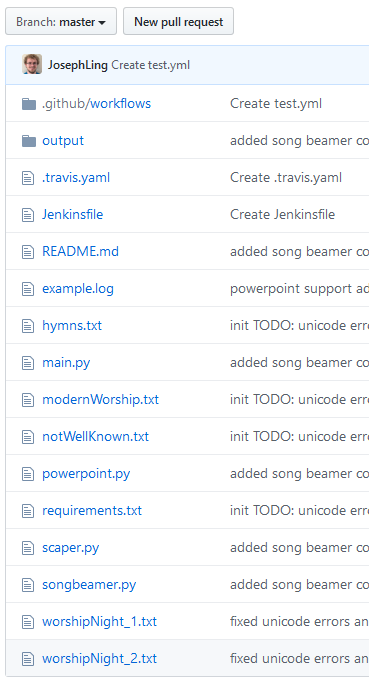
\includegraphics[scale=0.5]{repository file system.png}
    
    \caption[alt text]{Example Github repository that has multiple configuration types in it \cite{GithubRepoExample}. (This is an old repository that was reused in order to test out the scraper)}
    \label{image_example_repo}
  \end{minipage}%
  \hfill
  \begin{minipage}{.48\textwidth}
    \begin{verbatim}
      PATHS = {
        "travis": "travis",
        "gitlab": "gitlab-ci",
        "azure": "azure-pipelines",
        "appVeyor": "appveyor",
        "drone": "drone",
    
        "jenkinsPipeline": "jenkinsfile",
        
        "teamcity": ".teamcity/",
    
    
        "github": ".github/workflows/",
        "circleci": ".circleci/",
        "semaphore": ".semaphore/",
        "buildkite": ".buildkite/"
    }
    PATHS_MULTIPLE = ["github", "circleci", "semaphore",
     "teamcity", "buildkite"]
    NONE_YAML = ["jenkinsPipeline", "teamcity"]
    \end{verbatim}
    \caption{Python configuration file used to specify what types of configuration to search for. The key specifies the name of the configuration and the value is the location in the repository the config should be found.}
  \end{minipage}
\end{figure}

We chose to use a config file to specfiy which CI systems config files we would look for. If it was a directory then it would get all ".yaml" or ".yml" along with any Teamcity ".kts" and ".xml" files. However the script did not look into any of the sub directories which might be the cause for the low number of Teamcity configuration files found. In the case that it was a file that was on the top level directory we matched it the lowercase file name we found against the query.

In terms which configuration files to pick we based our list from Github Welcomes all CI Tools blog post in 2017 \cite{Github2017}. In addition we added Github Actions and Azure Pipelines to list as they are new potentially popular systems. 

\begin{figure}[h]
  \centering
  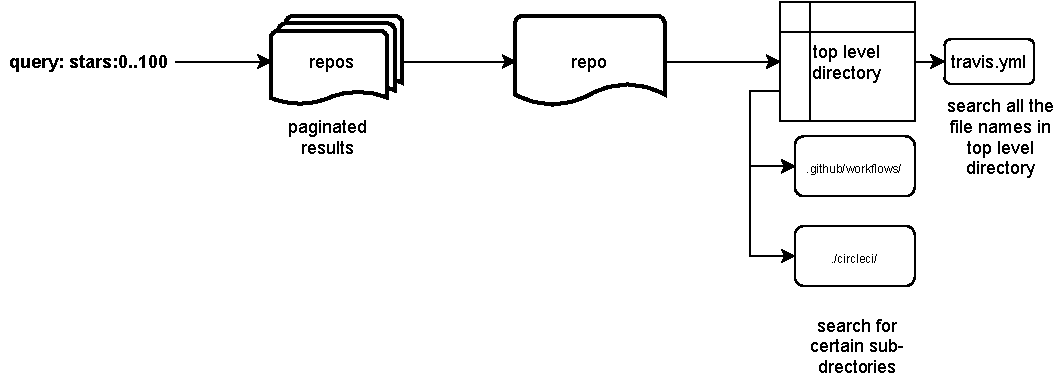
\includegraphics[width=\textwidth]{methadology diagram.pdf}
  
  \caption[alt text]{Diagram of the process used to search for projects with CI files in them}
  \label{image_methadolgoy_diagram}
\end{figure}

As can be seen in Figure \ref{image_methadolgoy_diagram} do a query based on the number of stars a project has on Github. This is because we need a way of getting a large sample from Github without introducing too much bais into the sample. That is not too say that our method is perfect but it provides an easy way to get a large sample that includes projects with and without CI.
Another potential solution would have been to use the "filename:travis.yaml" search api. However this did not provide information about which projects did not use CI. As well as for one unique search their can only be 1000 results returned by the Github Api. To mitigate that limit we search based stars as we did do a search for a 1000 results per star count. The limitation of this though was that there will be over a 1000 repositories that have 0 to 500 or even 500 to 501 stars. That means it is a sample that represents some of the population not a sample of all CI files on Github. 

As the config could have mistakes in it or we missed out a major CI system. We also saved the ReadMe.md when we scraped each project. A Readme.md is used to describe a project and will be displayed on Github at the bottom of the root directory. As can be seen in Figure \ref{ExampleGithubReadme} some ReadMe's have a label and/or links to the CI system used for that project. Therefore we also save that data when we scrape a project. 

\begin{figure}[h]
  \centering
  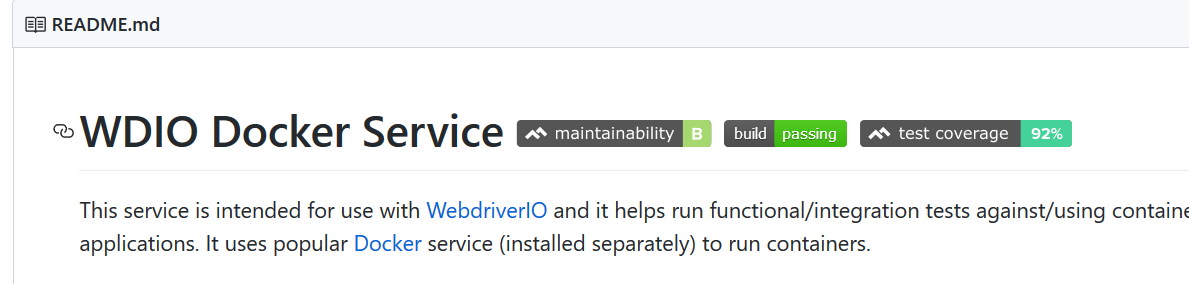
\includegraphics[scale=0.5, width=\textwidth]{2020-01-30-08-29-04.png}
  
  \caption[alt text]{Example of CI tag for Github ReadMe \cite{GithubReadMeExample}}
  \label{ExampleGithubReadme}
\end{figure}


We ended up with a config file with queries for configuration files for the following CI systems: Travis, Gitlab, Azure, App Veyor, Drone, Jenkins, Github, Circleci, Semaphore, Teamcity and buildkite. 

We excluded Wrecker from the search because they represented a very small number of projects in comparison to the other projects. As it seems since the Github survey in 2017 they got bought by Oracle and from doing a search on Github for what we think based on the docs \cite{WreckerDocs} and \cite{WreckerOpenSourceGithubSearch} for their config file naming convention. We were only able to find 20 results so did not include in the scraping script to speed up the process of searching for the other configuration file formats.

As can be seen later in on \ref{graph_scatter_stars_vs_subs} we weren't able to scrape the whole star count range easily. This is because the script would crash when Github gave a 500 error code at us randomly. Along with empty repositories initially causing a problem. In order to mitigate the damage of this the scraper would create a new Comma Separated Value (csv) file search e.g. one for stars:0..1 and another for stars:1..2. As all the csv file contained the same header we ran a script to combine all together at the end. Making sure to remove any duplicates by filtering on the Github project id.

% ------------------------------------------------------------------------------------------------------------------------------------
\section{Usage of CI}

\vspace*{-0.05in}
\subsection{What percentage of open-source projects use CI?}
\vspace*{-0.05in}


    \begin{table}[h]
\begin{tabular}{|l|l|l|l|l|}
\hline
    CI/CD & \textbf{count} & \textbf{repos with config} & \textbf{no. multiple} & \textbf{multiple percent}   \\ \hline
config file(s) &           12128     & 38.51\%                                & 1675          & 13.81\%             \\ \hline
found in ReadMe & 873     & 2.77\%                                &             &             \\ \hline
none found &            18493     & 58.72\%                                &             &             \\ \hline
\end{tabular}
\caption[Percentage of CI used for projects]{Percentage of CI used for projects}
\end{table}
    

\todo[]{hilton paper isn't the 34,000 just CI files though right? so CHECK }
\todo[]{what we want here is to explain what we have found and then do the comparison. Instead of throwing them into a comparison straight away without explaining the data }
Our sample of repositories is 31,494 in comparison to \citet{Hilton2016} which had a sample of 34,544. The percentage of CI projects they had was 40.27\%. As if you combined the "config file(s)" and "found in ReadMe". However in order to work out if a project might be using CI but the config file wasn't picked a search string is used. Therefore it is not as accurate as finding a config file as their could be false postives.
\todo[]{I am pretty sure it's 34,544 CI projects and so this paragraph needs to be rewritten if that is the case}

However that doesn't give us too much insight into the dataset. Here is a graph showing the subscribers plotted against the number of stars. The key here to understand is not potentially any correlation but to see the spread of data that the table is showing. 

\begin{figure}[!ht]
  \centering
  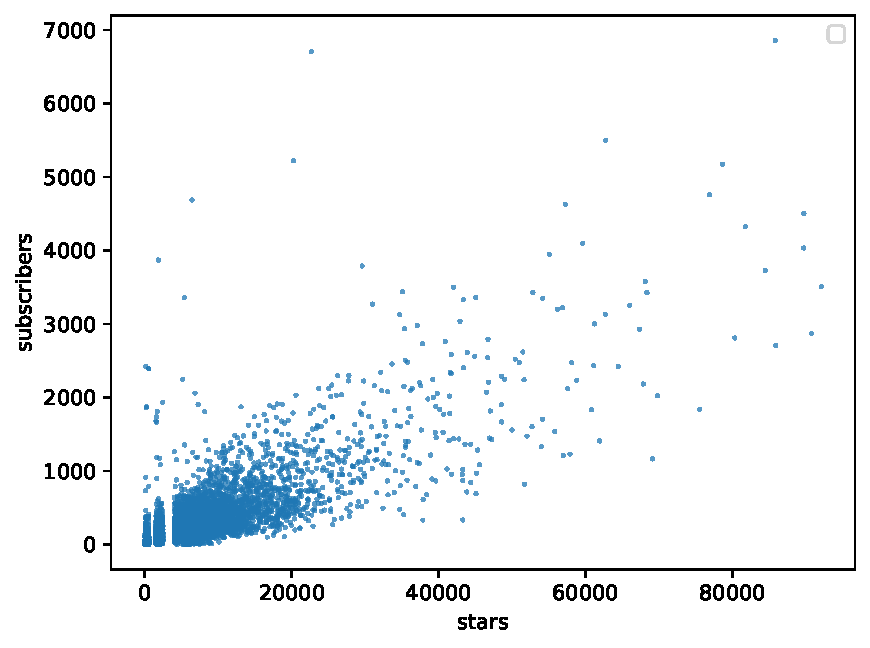
\includegraphics[width=\textwidth]{../src/results/sub vs stars.pdf}
  \caption[alt text]{Scatter graph of Github stars against subscribers}
  \label{graph_scatter_stars_vs_subs}
\end{figure}

Figure \ref{graph_scatter_stars_vs_subs} helps give a understanding to the give a depth of the data for where the graph is just blue. This is because on Github you get more repositories with smaller star counts than large ones.
In the case of two white bars at the lower end of the stars axis is where we do not have any data. This is due to time constraints on the paper and difficulties discussed in the Methodology (Section \ref{methodology}).

\begin{figure}[!ht]
  \centering
  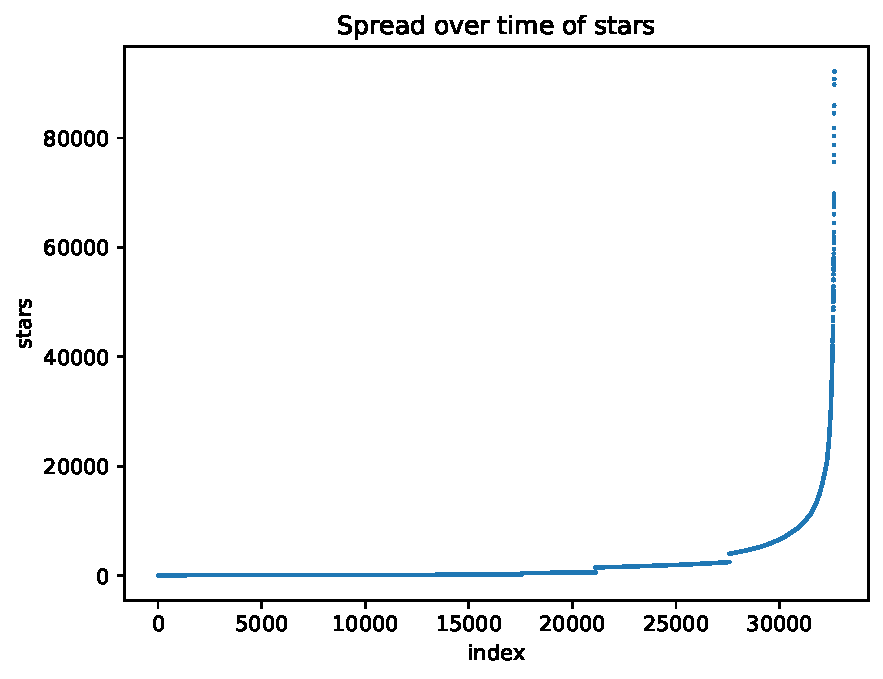
\includegraphics[width=\textwidth]{../src/results/spread over time.pdf}
  \caption[alt text]{Stars graph}
  \label{graph_scatter_stars_line}
\end{figure}

Figure \ref{graph_scatter_stars_line} provides insight into the density of the data for between 0 to 25000.
\todo[]{note the references are current to the figures but they are not playing ball with their position!!!}
\vspace*{-0.05in}
\subsection{What CI systems are projects using?}
\vspace*{-0.05in}
In Table \ref{table_config_types} we find like all other research Travis is the most popula0r CI system in use. However over the last 4 years since the \cite{Github2017} Circleci has lost out on it's rough quarter that it owned. In particular the rise of Github actions seems to have taken second place even though it is still very young in comparison (DATES). However this might not be down to the Circleci loosing out on their existing share. But potentially as the rise in CI usage goes up on Github. Projects are more likely to pick in the built in solutions to Github.
\begin {table}[!htbp]

\caption{Configuration types spread}
\label{table_config_types}
\begin{tabular}{lrl}
\hline
{} &  config & percentage \\ \hline

Travis          &   10607 &        74\% \\ \hline
Github          &    2301 &        16\% \\ \hline
CircleCi        &    1109 &         8\% \\ \hline
Jenkins pipeline &     161 &         1\% \\ \hline
Drone           &      84 &         1\% \\ \hline
Buildkite       &      32 &         0\% \\ \hline
Teamcity        &       4 &         0\% \\ \hline
Semaphore       &       2 &         0\% \\ \hline
Azure pipeline           &       1 &         0\% \\ \hline

\end{tabular}
\end{table}


Our sample of repositories is 31,494 this means that as it is a representation of projects on Github so won't account for the whole of it. This means that although Wrecker had the smallest count of CI when researching of 20 projects. In Table \ref{table_config_types} we have configuration types that have lower counts. This is because that search for the 20 searched the whole of Github but the scraping was only able to do a small sample. Additionally their potentially could be faults in the scraping causing it show such low numbers for the last 3.

\pagebreak
% ------------------------------------------------------------------------------------------------------------------------------------
\vspace*{-0.05in}
\subsection{Do certain types of projects use CI more than others?}  
\vspace*{-0.05in}

Below shows all the CI projects sorted then grouped together per 540 projects. Then in this case we choose to categories via star count for each project. 

\begin{figure}[!htbp]
  \centering
  \begin{minipage}{.48\textwidth}
    \centering
    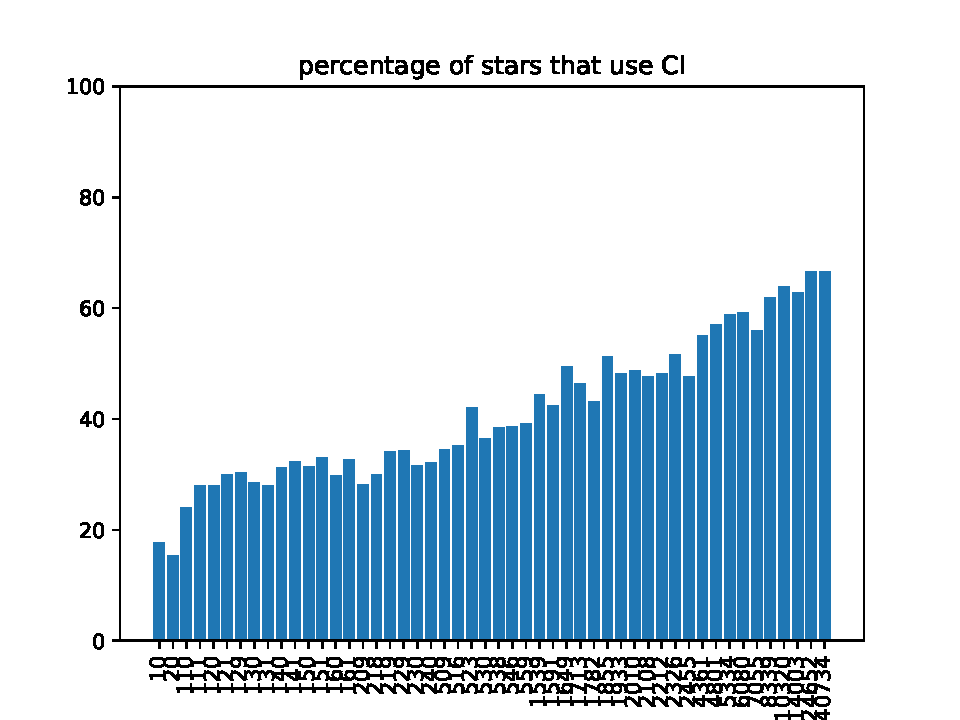
\includegraphics[width=.9\textwidth]{../src/results/percentage stars with CI.pdf}
    \caption{2020 dataset}
    \label{fig:test1}
  \end{minipage}%
  \hfill
  \begin{minipage}{.48\textwidth}
    \centering
    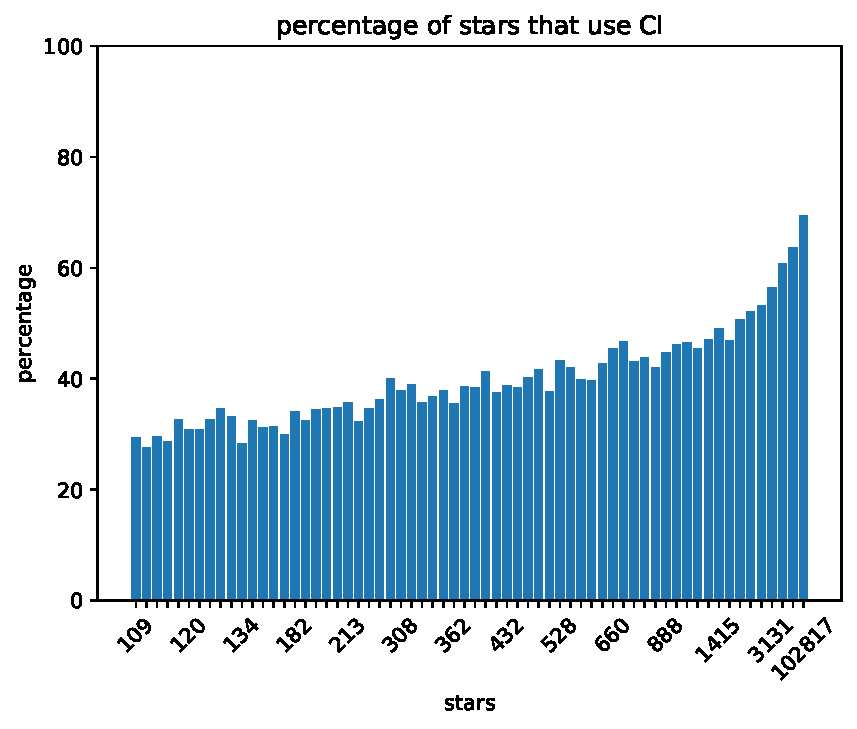
\includegraphics[width=.9\textwidth]{../src/results/percentage sub with CI other paper source.pdf}
    \caption[]{2016 dataset}
    \label{fig:test2}
  \end{minipage}
  \caption{In Figure \ref{fig:test1} is the results from this research and in Figure \ref{fig:test2} is the results from \cite{Hilton2016}.}
\end{figure}

Here in Figure \ref{fig:test1} and \ref{fig:test2} we are comparing whether or not in the last 4 years the number of stars increases the CI being used. Their seems to a steeper gradient in the more recent datasets. However as \ref{fig:test1} starts at zero stars and \ref{fig:test2} starts at 100 stars their is signifacant dip at the start of the first graph.

\begin{figure}[!h]
  \centering
  % TODO: make this bigger when the time comes
  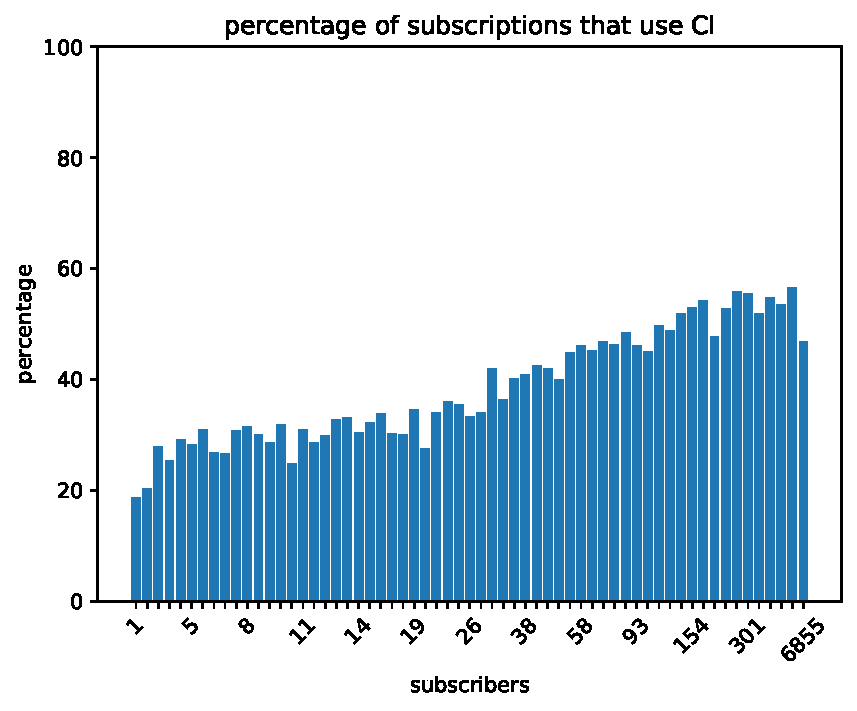
\includegraphics[width=.8\textwidth]{../src/results/percentage sub with CI.pdf}
  \caption{Subs graph}
  \label{graph_percentage_subs}
\end{figure}
\todo[]{when the writing is good and nearly polished make this the proper size}
Figure \ref{graph_percentage_subs} uses the same method as Figure \ref{fig:test1} except is does it based the number of subscribers. Subscribers are used on Github to keep update on the changes on the project. This could range from core team members working on the project to people that want to be notified about a new release. 
In looking at this metric the hypothesis was that it would have a sharper rise in percentage of projects using CI per subscriber. However that was not the case overall the gradient is not as strong. There is no comparison to \cite{Hilton2016} because their final corpus does not contain subscriber count for each project.



\begin{figure}[!h]
  \centering
  % TODO: make this bigger when the time comes
  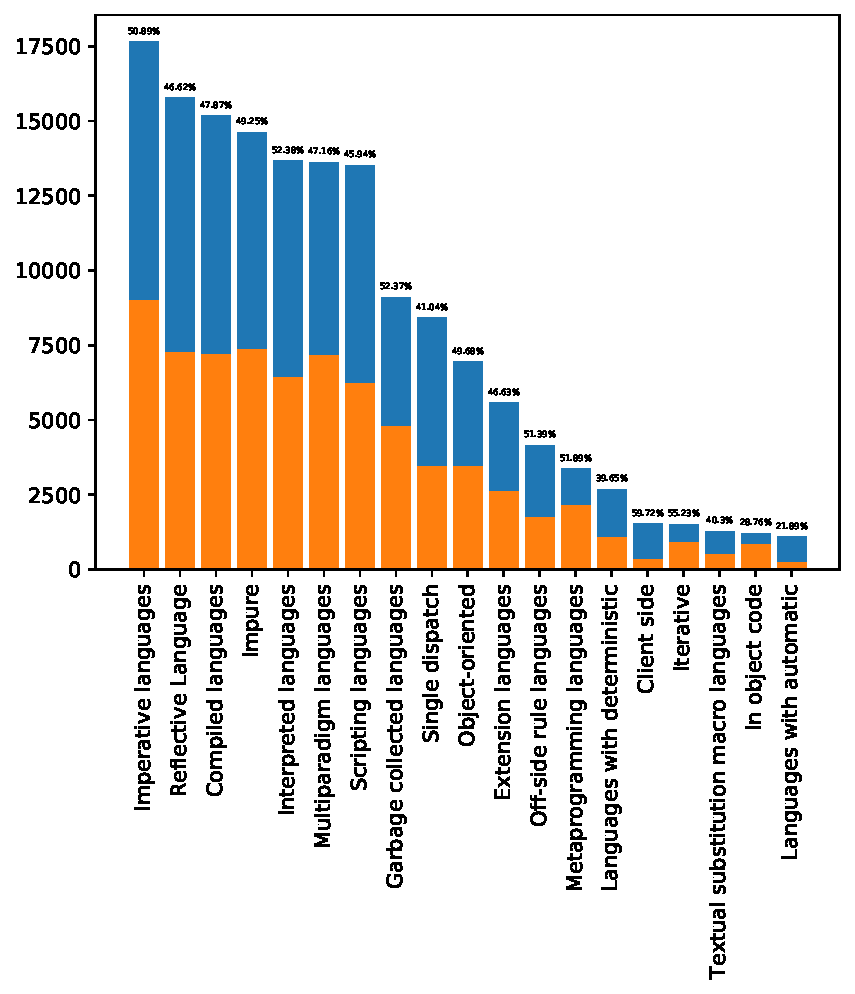
\includegraphics[width=.8\textwidth]{../src/results/languages.pdf}
  \caption{Subs graph}
  \label{graph_langs}
\end{figure}

\begin{table}
\centering
\caption{Total count of all programming languages used by projects. It has programming languages that only found once removed.}
\label{table:languages}
\begin{tabular}{|l|r|r|r|}
\hline
{} &  total language count &  using CI &  percentage CI \\

b'ASP'              &                     7 &       NaN &            NaN \\
b'ActionScript'     &                    21 &       2.0 &       9.523810 \\
b'AppleScript'      &                     6 &       NaN &            NaN \\
b'Arduino'          &                    21 &       NaN &            NaN \\
b'Assembly'         &                    47 &      18.0 &      38.297872 \\
b'AutoHotkey'       &                     6 &       NaN &            NaN \\
b'Batchfile'        &                    18 &       2.0 &      11.111111 \\
b'C\#'               &                   943 &     180.0 &      19.088017 \\
b'C'                &                  1278 &     515.0 &      40.297340 \\
b'C++'              &                  1571 &     821.0 &      52.259707 \\
b'CMake'            &                    17 &       6.0 &      35.294118 \\
b'CSS'              &                   650 &     143.0 &      22.000000 \\
b'Clojure'          &                   148 &      74.0 &      50.000000 \\
b'CoffeeScript'     &                   127 &      60.0 &      47.244094 \\
b'Common Lisp'      &                    27 &       3.0 &      11.111111 \\
b'Coq'              &                     7 &       7.0 &     100.000000 \\
b'Crystal'          &                    13 &      16.0 &     123.076923 \\
b'Cuda'             &                    15 &       2.0 &      13.333333 \\
b'D'                &                     8 &       5.0 &      62.500000 \\
b'Dart'             &                   168 &      39.0 &      23.214286 \\
b'Dockerfile'       &                    54 &      20.0 &      37.037037 \\
b'Eagle'            &                     7 &       1.0 &      14.285714 \\
b'Elixir'           &                    67 &      55.0 &      82.089552 \\
b'Elm'              &                    19 &      12.0 &      63.157895 \\
b'Emacs Lisp'       &                   104 &      44.0 &      42.307692 \\
b'Erlang'           &                    68 &      41.0 &      60.294118 \\
b'F\#'               &                    24 &      17.0 &      70.833333 \\
b'Fortran'          &                     7 &       5.0 &      71.428571 \\
b'GLSL'             &                     9 &       1.0 &      11.111111 \\
b'Go'               &                  1512 &    1184.0 &      78.306878 \\
b'Groovy'           &                    37 &      26.0 &      70.270270 \\
b'HCL'              &                    20 &       4.0 &      20.000000 \\
b'HTML'             &                   856 &     205.0 &      23.948598 \\
b'Haskell'          &                   121 &      84.0 &      69.421488 \\
b'Haxe'             &                    12 &       5.0 &      41.666667 \\
b'Java'             &                  2963 &    1108.0 &      37.394533 \\
b'JavaScript'       &                  6663 &    3323.0 &      49.872430 \\
b'Julia'            &                    40 &      65.0 &     162.500000 \\
b'Jupyter Notebook' &                   459 &      63.0 &      13.725490 \\
b'Kotlin'           &                   284 &     150.0 &      52.816901 \\
b'Lua'              &                   122 &      37.0 &      30.327869 \\
b'MATLAB'           &                    14 &       3.0 &      21.428571 \\
b'Makefile'         &                    49 &      14.0 &      28.571429 \\
b'Matlab'           &                    35 &       1.0 &       2.857143 \\
b'Nim'              &                    11 &       4.0 &      36.363636 \\
b'Nix'              &                     7 &       2.0 &      28.571429 \\
b'OCaml'            &                    33 &      31.0 &      93.939394 \\
b'Objective-C'      &                  1087 &     239.0 &      21.987121 \\
b'Objective-C++'    &                    15 &      11.0 &      73.333333 \\
b'OpenSCAD'         &                     6 &       NaN &            NaN \\
b'PHP'              &                  1337 &     806.0 &      60.284218 \\
b'PLpgSQL'          &                    10 &       4.0 &      40.000000 \\
b'Pascal'           &                    21 &       2.0 &       9.523810 \\
b'Perl'             &                    85 &      35.0 &      41.176471 \\
b'PowerShell'       &                    88 &       6.0 &       6.818182 \\
b'Processing'       &                     6 &       NaN &            NaN \\
b'Puppet'           &                     6 &       2.0 &      33.333333 \\
b'Python'           &                  4127 &    1726.0 &      41.822147 \\
b'QML'              &                    13 &      12.0 &      92.307692 \\
b'R'                &                   129 &      86.0 &      66.666667 \\
b'Reason'           &                     7 &       3.0 &      42.857143 \\
b'Rich Text Format' &                    14 &       2.0 &      14.285714 \\
b'Roff'             &                    15 &       5.0 &      33.333333 \\
b'Ruby'             &                  1053 &     732.0 &      69.515670 \\
b'Rust'             &                   352 &     333.0 &      94.602273 \\
b'Scala'            &                   223 &     162.0 &      72.645740 \\
b'Scheme'           &                     8 &       2.0 &      25.000000 \\
b'ShaderLab'        &                    10 &       NaN &            NaN \\
b'Shell'            &                   816 &     244.0 &      29.901961 \\
b'Smarty'           &                     9 &       5.0 &      55.555556 \\
b'Swift'            &                   733 &     350.0 &      47.748977 \\
b'TSQL'             &                    15 &       4.0 &      26.666667 \\
b'TeX'              &                    89 &      18.0 &      20.224719 \\
b'TypeScript'       &                   900 &     779.0 &      86.555556 \\
b'Vala'             &                    11 &       6.0 &      54.545455 \\
b'Verilog'          &                     8 &       NaN &            NaN \\
b'Vim script'       &                   161 &      60.0 &      37.267081 \\
b'VimL'             &                    35 &       NaN &            NaN \\
b'Vue'              &                   186 &      58.0 &      31.182796 \\
b'XSLT'             &                     7 &       1.0 &      14.285714 \\

\end{tabular}
\end{table}


 
\pagebreak
% ------------------------------------------------------------------------------------------------------------------------------------
\section{Structure of configuration files}

\vspace*{-0.05in}
\subsection{What are the common errors when loading yaml configuration?}
\vspace*{-0.05in}

\begin{figure}[!ht]
  \centering
  \begin{minipage}[t]{.48\textwidth}
    \textbf{Composer error}
    In the example it has two steps that are using an yaml anchor. This allows for the yaml to be referenced somewhere else. However if you define the anchor twice with the same name it causes an composer error. As you have two references using the same name so it won't know which one to use.
  \end{minipage}%
  \hfill
  \begin{minipage}[t]{.48\textwidth}
    \begin{verbatim}
      definitions: 
      steps:
      - step: &build-test
      name: Build and test
      script:
      - mvn package
      - step: &build-test
      name: deploy
      script:
      - ./deploy.sh target/my-app.jar
    \end{verbatim}
  \end{minipage}
\end{figure}

\begin{figure}[!h]
  \centering
  \begin{minipage}[t]{.48\textwidth}
    \textbf{Scanner error}
    The first step of loading the yaml is to scan it to create the tokens. However invalid characters such as "\textbackslash t" are invalid. 
  \end{minipage}%
  \hfill
  \begin{minipage}[t]{.48\textwidth}
    \begin{verbatim}
      definitions: \t
    \end{verbatim}
  \end{minipage}
\end{figure}
\begin{figure}[!ht]
  \centering
  \begin{minipage}[t]{.48\textwidth}
    \textbf{Parse error}
    In this example it has scanned the file and created tokens for the syntax. Now it parses the syntax and works out if each token is valid given it's current context. In this case a closing ] without an opening [ is invalid.
  \end{minipage}%
  \hfill
  \begin{minipage}[t]{.48\textwidth}
    \begin{verbatim}
      definitions: ]
    \end{verbatim}
  \end{minipage}
\end{figure}

\begin {table}[!htbp]

\caption{cats}
\begin{tabular}{|l|l|l|l|}
\hline
\textbf{yaml\_encoding\_error} &  composer error &  parse error &  scanner error \\ \hline
\textbf{config  } &                 &              &                \\ \hline

\textbf{circleci} &               0 &            0 &              1 \\ \hline
\textbf{drone   } &              30 &            0 &              0 \\ \hline
\textbf{github  } &               0 &            0 &              3 \\ \hline
\textbf{travis  } &               6 &           10 &             21 \\ \hline

\end{tabular}
\end{table}


As can be seen in the Table \ref{table_yaml_errors} their our configuration files with yaml errors meaning that the CI for that project will not load. Yet it seems that a very small percentage of projects that have them. For example the two highest configuration types with errors are Drone (36.90\%) followed by Travis (0.348\%).

In the case for Drone all the errors are for the same type of error. Potentailly this could be because of how anchors are a lot more common in Drone.

For Travis as it is the largest config type out of the sample by a signifacant amount it is more likely to contain more errors. Yet with such a small amount it seems like yaml errors aren't a major problem in CI. Although as they are required to be fixed in order for the CI to run the chances are the ones with errors ones that are being changed when the scraping was being done. Meaning that as the CI has been set up correctly for the other 99.632\% as they are not needing to change because their our no yaml errors in it and presumbely it is doing what they intend for it to do.


\pagebreak

\begin{figure}[!ht]
  \vspace*{-0.05in}
  \subsection{How are comments used in configuration?}
  \vspace*{-0.05in}
\end{figure}


The assumption was the as continuous integration setups can be complicated and have edge cases. Therefore comments would be used to describe and handle that complexity.

An example configuration file below for Github actions using the default template slightly altered. Shows two examples of comment usage, the first being including useful information about why a particular version of the programming language was chosen. The second is that the tests have been disabled by commenting them out. 



\begin{figure}[!htbp]
  \centering
  \begin{minipage}[t]{.48\textwidth}
    In order to pick up on all these different types of comments. All the CI files were parsed and then regular expressions were used to pick on up key factors such as "note:". Along with multiple single line comments which made up a block/multi-line comment.
    
    For example in to the left there is an example Github Action yaml file. If were it would be parsed we would get: one multi line comment, 15 lines of code, 1 single line comment, a total of 5 comments and 20 lines in the file. Therefore their is a their is a ratio of 4:1 for code in this config file.
  \end{minipage}%
  \hfill
  \begin{minipage}[t]{.48\textwidth}
    \begin{verbatim}
      name: Python package
      on: [push]
      jobs:
      build:
      runs-on: ubuntu-latest
      steps:
      - uses: actions/checkout@v2
      - name: Set up Python
      uses: actions/setup-python@v1
      # note: only works with python 3
      with:
      python-version: 3.8
      - name: Install dependencies
      run: |
      python -m pip install --upgrade pip
      pip install -r requirements.txt
      #      - name: Test with pytest
      #        run: |
      #          pip install pytest
      #          pytest ./src
    \end{verbatim}
  \end{minipage}
\end{figure}

% NOTE: NEED TO EXPLAIN CODE_WITH_COMMENTS

Initially before we look at the comments it is important to understand how the rest of the file is made up. In the graph below (Figure \ref{fig:bar_comments_lines}) it shows how each configuration type is made up by mean of each part of the file. For all the yaml based configurations lines of code and number of lines in total are very close. Then for the number of comments being very very small on average.

In the case for Jenkins pipelines and teamcity there is a much higher usage of having code with comments. 


\begin{figure}[!ht]
  \centering
  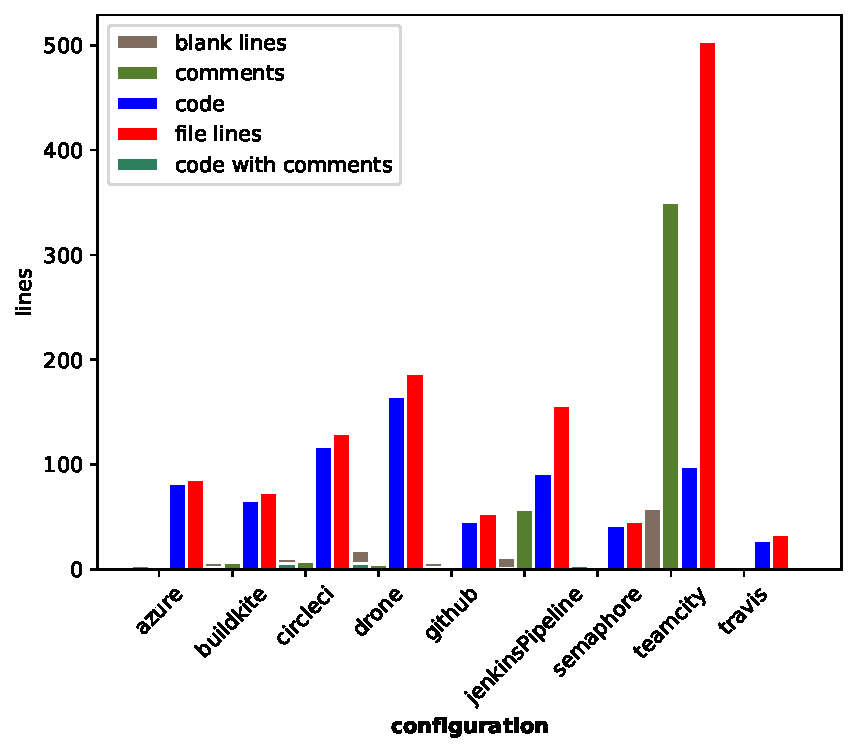
\includegraphics[width=\textwidth]{../src/results/basic comments bars.pdf}
  \caption[alt text]{Mean of line counts}
  \label{fig:bar_comments_lines}
\end{figure}

Ratios:
\begin{itemize}
  \item{code: comments}
  \item{code: line total}
  \item{code: blank lines}
  \item{single line comment: multiline comment}
  \item{single line comment: code with comment}
\end{itemize}






\begin{figure}[!ht]
  \centering
  \begin{minipage}[!t]{.48\textwidth}
    In Figure \ref{fig:comment_types} a regular expression was used to label the comments. There were key different types of comment that we wanted to find. The first being the commented out code which we did by searching for version numbers in commments. The second being useful information about the structure of the CI file such todo, note, importanat comments (e.g. //todo). In order to increase the search for this we included searching for urls and seperation comments (e.g. //===).
    
  \end{minipage}%
  \hfill
  \begin{minipage}[!t]{.48\textwidth}
    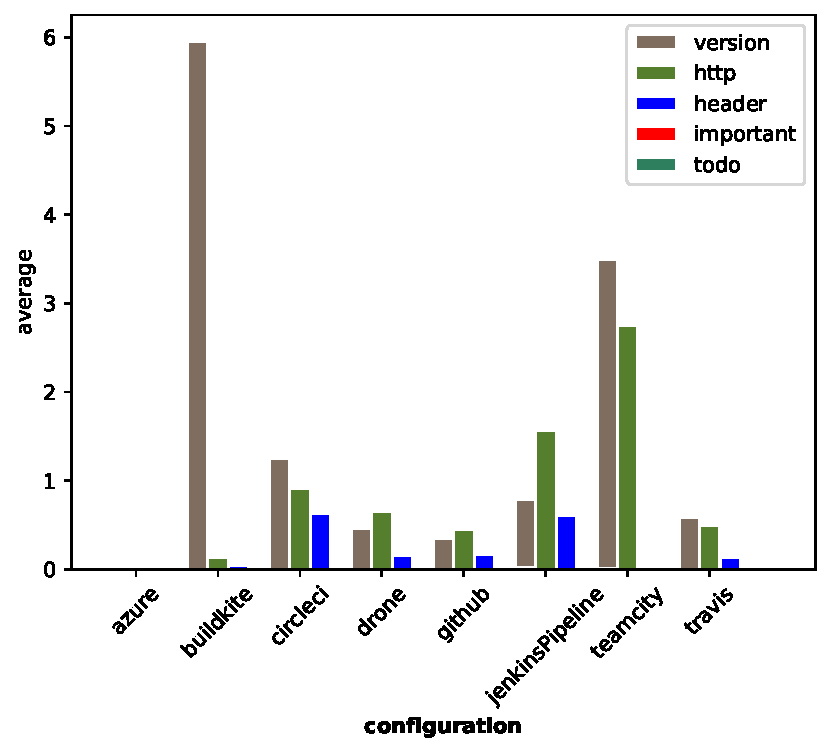
\includegraphics[width=\textwidth]{../src/results/comments usage bars.pdf}
    \caption[alt text]{Comment types}
    \label{fig:comment_types}  
  \end{minipage}
\end{figure}

From labelling the comments in Figure \ref{fig:comment_types} we can see that having comments with versions in and urls is most common. This could indicate comments from templates or how they are commented. Although yet again the amount of labels found on average is still very low.

Overall we have found that comments are not used a lot. In the cases that they are used it's more likely to be from a configuration template or commenting out configuration.
% NOTE: update this when raitos are done

\pagebreak

\vspace*{-0.05in}
\subsection{Are external scripts used within the configuration?}
\vspace*{-0.05in}

An external script is a bash or powershell script typically depending on the operating system. It can be used to build, deploy or do any step that CI takes. The key difference between it and the CI configuration is that it be executed on a users machine. Therefore you do get some setups where you have scripts defined for building and deploying the code that the users and CI both use. Most CI systems allow for "script" tags to be used which could be described as an internal script. Therefore external scripts are defined outside the CI configuration in the directory.

The methodology we used to handle this was too look at how many bash or powershell scripts where used in CI. Using the code the parsed the yaml files for comments we were able to check do a using a regular expression for either of those files.  


\begin{figure}[!ht]
  \centering
  \begin{minipage}[!t]{.48\textwidth}
      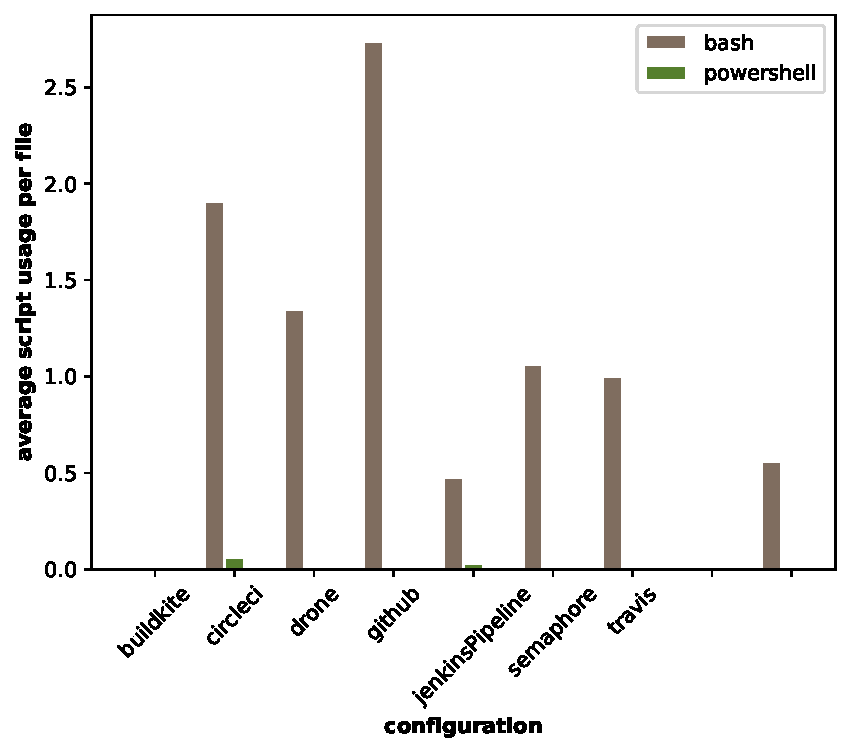
\includegraphics[width=\textwidth]{../src/results/scripts usage bars.pdf}
      \caption[alt text]{Comment types}
      \label{fig:script_usage}  
  \end{minipage}%
  \hfill
  \begin{minipage}[!t]{.48\textwidth}
    

\caption{sum of scripts used}
\label{table:scripts used}
\begin{tabular}{|l|l|l|}
\hline
{} &  bash &  powershell \\ \hline

\textbf{buildkite      } &    61 &           2 \\ \hline
\textbf{circleci       } &  1497 &           8 \\ \hline
\textbf{drone          } &   230 &           0 \\ \hline
\textbf{github         } &  1097 &          65 \\ \hline
\textbf{jenkinsPipeline} &   171 &           0 \\ \hline
\textbf{semaphore      } &     2 &           0 \\ \hline
\textbf{travis         } &  5937 &           3 \\ \hline

\end{tabular}


  \end{minipage}
\end{figure}

asdf
In Figure \ref{fig:script_usage} we have the average number of times a script is used for a configuration file that already has a script being used.

As some of the necessary actions are being done in the scripts and not in the CI file. Potentially there could be less lines of code in the configuration for files that use scripts. However in Figure \ref{fig:script_scatter_lines} we can see that the data is very spiky with outliers. Then in Figure \ref{fig:script_scatter_lines2} we can see the same affect when trying to see if the more popular a project is affects the chances of it using CI.

\begin{figure}[!ht]
  \centering
  \begin{minipage}[!t]{.48\textwidth}
    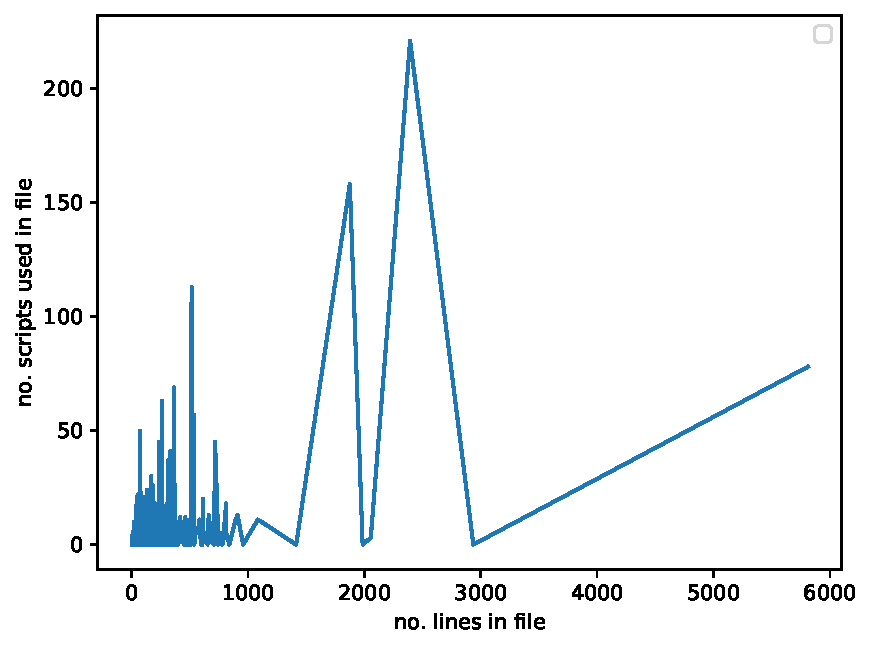
\includegraphics[width=\textwidth]{../src/results/scripts vs lines.pdf}
    \caption{no. scripts to no. lines}
    \label{fig:script_scatter_lines}    
  \end{minipage}%
  \hfill
  \begin{minipage}[!t]{.48\textwidth}
    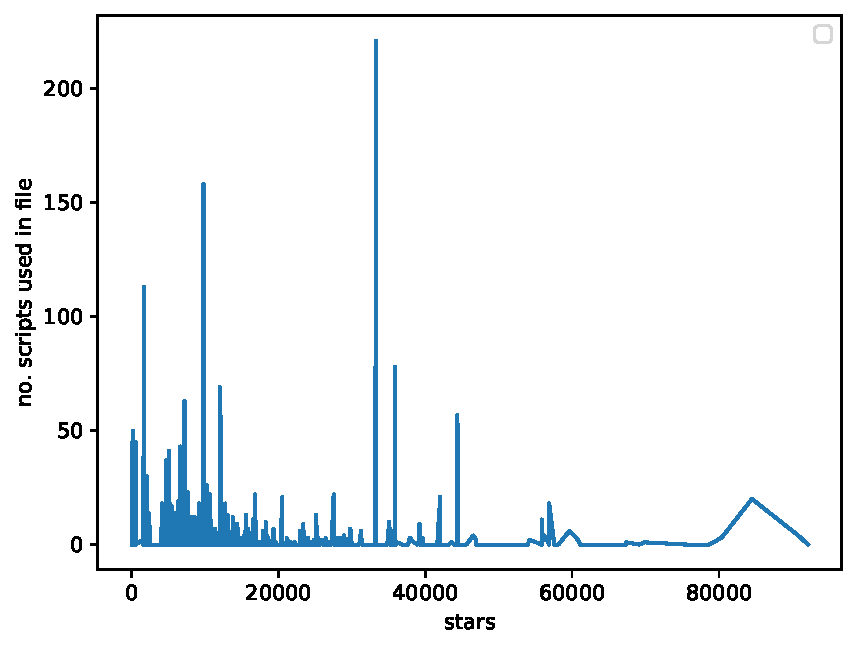
\includegraphics[width=\textwidth]{../src/results/scripts vs stars.pdf}
    \caption{no. scripts to stars}
    \label{fig:script_scatter_lines2}
  \end{minipage}
\end{figure}

\todo[]{percentage of usage needed like we had for comments}
Overall we can see that scripts are not used that much. And their no correlation between lines of code and usage of external scripts.


\pagebreak

\section{Threats to validatity}

The major and most obivious threat is the sample gathered from scraping the data from Github. This has already been touched on in the \ref{methodology} section but now we are going to look at it in more detail.

Firstly if we assume that the scraping works perfectly then it's only at maximum a 1000 open source projects per star. That is excluding closed source projects which would range from personal projects to companies. As well as it is only data from Github not from Gitlab, bitbucket or other version control hosting services. This leads to bais in the data for example if Gitlab was also scraped then we would get a lot more Gitlab ci files. However in order to get best spread of data Github has the best api and most services do not tie you down to use only their service. As well although we could get a 1000 projects per star we were still able to get around 30,000 projects and a wide spread across Github. The key aspect being that because it was a sample we focused on getting a good spread of data.

Secondly the scraping script is not perfect in how it finds configuration files. As it only looks in the top level directory for the file name pattern described in their docs or unique folder. Therefore if the systems allowed many different names or different names in past it wouldn't have picked it CI system. Additionally we only decided to scrape for certain CI files. Yet we chose a good scope based on previous research into the top CI files. As well the scraping script has been tested worked on to try and minimise any bugs. In the case that we did not pick up a CI file we ran a regexp against the ReadMe file to get a better understanding of the error bounds.

Thirdly identifying which projects are programming projects or would have a need for CI. Based on the research \cite{Kalliamvakou2014} it is important to filter out repositories that aren't part of the question being asked. Therefore we could have looked to try and filter out Github static sites and other none software based projects. However if assume a certain type of project won't be using CI then we would be introducing bais when trying to answer how CI is used. For further research better labelling of what kind of projects are which would potentially beneficial though.

% From methadolgoy to work out how to fit in:
% There are dangers in scraping data off Github in terms of assumptions to do with the population as found in \cite{Kalliamvakou2014}. Our dataset does not contain any forked repositories. But due to time constraints number of commits and frequency of recent commits has not been looked at. This would be an interesting area of further research in order to improve the quality of the sample but also to look at how that affects the frequency of CI usage.

% Additionally the assumption that all repositories are of programming projects with code in them is wrong. A number of repositories can be used for storage, experimental, academic and other things. However they to all some extent can use CI/CD for their work as a number of books were found when looking through the dataset could use CI/CD.



% strength and validaltiy section 
% - possible issues
% - baise assume in the data
% - e.g. sampling vai star
% - focusing on Github
% - problematic of scraping tool


\pagebreak



\section{Summary}

We got a sample of XXXX open source projects from Github and were able to compare that to a previous study 4 years ago. In doing so we found that usage of CI projects was similar and that more popular a project the higher chance it would be using CI. This lined with the research from 4 years ago. The major change was the increase in popularity of Github Actions taking over second place from Circleci. Additionally we look at whether or not the number of people watching the project had the same effect. It did but to a lesser extent.

In terms of structure of CI configuration we looked each line of was used in context of comments. We found that a very few projects use comments in their CI. In terms of how they used scripts, we found the majority of projects do not use external scripts. 

From this a better understanding of this topic could be gathered by looking into the data gathered more. As we found we were faced with a lot more questions while doing this research as we go into below.

\vspace*{-0.05in}
\subsection{Discussion and further research}
\vspace*{-0.05in}
In the process of writing this paper we kept on considering more research questions. As there is a lot of meta data that you can get for a single project, in addition to what was used for this paper.

Further research into usage that we would like to do is look into how the size of the project affects the chance that it uses CI. Then looking at the usage of scripts within CI configuration, for example using a script tag to run a shell script. As while doing the research we found some projects use scripts a lot while others just used the CI config. This would lead to questions around which CI system has a higher amount of scripts used. But also looking at how much they enable them to be used and what is the size of those scripts.
The data for the programming language and version(s) is in the config. Therefore it would be possible to work out how much usage each version is getting of a particular programming language.

Further research into structure could look into the naming of each part of the build process that is used. This would be interesting as it would provided insight into what terms are commonly used. As well an idea into how people plan or don't plan out their configuration files.
Additionally CI systems can be designed to run on every commit to version control or only commits to certain branches. Therefore by looking at the branching regexp that are being used an better understanding of how branches are actually used in software development where CI is also used could be found out. In particular looking into which branching method (e.g. \citet{BranchGITFLOW2010}, \citet{BranchGITHUBFLOW2017}, \citet{BranchTrunk2013}) is used more for projects with CI and those that don't. 
asdf
In addition working on pruning our dataset using methods outlined in \cite{Kalliamvakou2014}. 

% After looking at these results three areas of research that could be interesting would be filtering the sample to only projects that had recent commits. On the assumption that CI is becoming more popular and stale projects won't require CI.

% Looking into whether or not that assumption is the case. Then looking commit count to see if projects with more commits are more likely to use CI.

\section{Acknowledgement}
We wish to thank Michael Hilton in particular for providing the corpus for their research \cite{Hilton2016}. 

% \appendix
% \section*{Appendix A. Probability Distributions for N-Queens}


[section ommitted]



\vskip 0.2in
\bibliography{sample}
\bibliographystyle{kentHarvard}

\end{document}
